\documentclass[conference,compsoc]{IEEEtran}
\usepackage{graphicx}
\usepackage{hyperref}
\hypersetup{
    colorlinks=true,
    linkcolor=blue,
    filecolor=magenta,      
    urlcolor=blue,
}
\urlstyle{same}

\ifCLASSOPTIONcompsoc
  % IEEE Computer Society needs nocompress option
  % requires cite.sty v4.0 or later (November 2003)
  \usepackage[nocompress]{cite}
  
  
\else
  % normal IEEE
  \usepackage{cite}
\fi

% correct bad hyphenation here
\hyphenation{op-tical net-works semi-conduc-tor}


\begin{document}
\title{Graph Bandwidth Problem}

\author{\IEEEauthorblockN{Maaz Saeed}
\IEEEauthorblockA{Dhanani School of Science\\and Engineering\\
Habib University\\
Karachi - 75290, Sindh, Pakistan\\
Email: @st.habib.edu.pk}
\and
\IEEEauthorblockN{Muhammad Usaid Rehman}
\IEEEauthorblockA{Dhanani School of Science\\and Engineering\\
Habib University\\
Karachi - 75290, Sindh, Pakistan\\
Email: mr04302@st.habib.edu.pk}
\and
\IEEEauthorblockN{Maham Shoaib Patel}
\IEEEauthorblockA{Dhanani School of Science\\and Engineering\\
Habib University\\
Karachi - 75290, Sindh, Pakistan\\
Email: mp04911@st.habib.edu.pk}}

\maketitle

\begin{abstract}
The abstract goes here.
\end{abstract}


\IEEEpeerreviewmaketitle

\section{Introduction} \label{intro}
% no \IEEEPARstart
Bandwidth is a basic, fundamental concept in Graph Theory, relating to almost any and every mathematical property possessed by a graph. The bandwidth of a graph refers to it's minimum bandwidth under any ordering; the bandwidth of the ordering of a graph is the maximum distance between two adjacent vertices.
\\
\\
The inception of the Matrix Bandwidth Problem, occurred in the 1950s, when structural engineers attempted to analyze steel frameworks by their structural matrices, via computerized manipulation. The term 'bandwidth' was birthed as the engineers had endeavoured to discover a matrix in which all the non-zero elements lay withing a narrow 'band'. The inspiration for this came from operations such as inversion or finding determinant in as little time as possible.
\\
\\
In 1962, similar to this approach, L.H Harper, and A.W Hales conceived the bandwidth, and bandwidth sum. They used edge differences to represent single errors in a 6-bit picture code, in a hypercube, where it's vertices were words of the code \cite{10.2307/2946514}. Some time after this, R.R Kohrfage initialized his work on the graph bandwidth problem \cite{ccdg1982}. Finally, F. Harary published the problem, as we know it today, officially \cite{https://doi.org/10.1002/bimj.19660080427}.
\\
\textbf{Key terms:} Graph Theory, Bandwidth, Evolutionary Algorithms
 
\hfill May 26, 2021

\subsection{Problem Definition}
Let's define the problem in more formal terms with some added notation. 
The mapping $f$ is defined as $f: V(G) \to \{1, 2, \dots, n\}$, where $n = |V|$ -- also called a \emph{perfect numbering}. \cite{Lee2016} Therefore, 
we can think of these mappings as essentially orderings of the vertices. The bandwidth of an ordering is defined as:
\begin{equation}
B_f(G) = \max_{uv \in E(G)}\{|f(u) - f(v)|\}.
\end{equation}

\begin{equation}
  v_{ij}(t+1) = v_{ij}(t) + c_1r_{1j}(t)[y_{ij}(t)-x_{ij}(t)] + c_2r_{2j}(t)[\hat{y}(t) - x_{ij}(t)]
\end{equation}

The bandwidth of the graph $G$ is given by the bandwidth of the best possible ordering:
\begin{equation}
B(G) = \min\{B_f(G): f\; is\; a \;numbering\; of\; G\}.    
\end{equation}
We will be restricting ourselves to working with perfect numbering.

\section{Preliminary Concepts}
\subsection{Evolutionary Algorithms}
Evolutionary Algorithms (also known as Genetic Algorithms) is a term referring to a family of algorithms based on the evolution we see around us, in nature. By mimicking learning, natural selection, reproduction, we can produce solutions for various search and optimization problems. This concept of evolving algorithms enables us to bypass the setbacks of traditional search / optimization algorithms.

\subsubsection{Darwinian Evolution}
Evolutionary Algorithms are derived of a simplified Darwinian evolution. The principles of such a cycle can be as such:
\begin{enumerate}
    \item \textbf{Variation} - Individual members of a given population may have differing attributes from one another, for example, physical appearance.
    \item \textbf{Inheritance} - Offspring resemble their parents to certain extents. In this manner, traits are passed down from one generation to another; unrelated individuals are less likely to have common traits, as compared to them with their family trees.
    \item \textbf{Selection} - Nature follows 'survival of the fittest' ideology. Individuals that are better able to locate and make use of resources compared to their peers, are more likely to survive in their respective environments. 
\end{enumerate}
In accordance with these principals, results that we obtain from our algorithm may or may not resemble those of previous iterations. With careful manipulation of parameters, solutions produced by our code can be ranked higher or lower than others.
\subsubsection{Analogies}
Where Darwinian evolution maintains a population of individual solutions, genetic algorithms maintain \textbf{individuals} - a population of candidate solutions \cite{Wiransky-GA}. The theory behind these algorithms is that solutions are produced, and improved upon, by iteratively re-producing newer generations of solutions.
\\
The various components of an evolutionary algorithm are as follows:
\begin{enumerate}
    \item \textbf{Genotype} - In nature, genotypes are collections of genes. When two individuals procreate, a mixture of genes from both, will make up the chromosomes of the offspring. In code, these \textbf{chromosomes} can be expressed, for example, as strings in binary. 
    \item \textbf{Population} - Population refers to the collection of chromosomes. At any given moment, the algorithm will maintain a population of individuals - candidate solutions for the problem that is being attempted to be solved. In a nutshell, it is the current generation, which will be replaced by the next generation of offspring. 
    \item \textbf{Fitness Function} - a function used to evaluate individuals in a given population. Individuals that produce better results, will be more favoured when it comes to selection for breeding of newer generations. As this cycle runs, individuals display continuous improvement until a satisfactory solution to our problem is found, at which point we can terminate the operation.
    \item \textbf{Selection} - After individuals are evaluated and awarded a \textit{fitness value}, the best among them are chosen to breed and produce the newer generation. It is important to note that individuals with lower scores are still selected, but with lower probabilities, so as to not cause extinction of their respective attributes.
    \item \textbf{Crossover} - refers to the mixing of chromosomes of the two parent individuals that were paired in the selection process to produce two new chromosomes (offspring). This process is also known as recombination.
    \item \textbf{Mutation} - fulfills the purpose of periodically (at random; not in a set pattern) refreshing the population. This introduction of new patterns in the chromosomes encourages the algorithm to search in unexplored areas, rather than just exploiting what it has already chartered. The mutation may occur as random changes in chromosomes, for example, in binary string representation, a single bit may be switched.
\end{enumerate}
\paragraph{}
\begin{center}
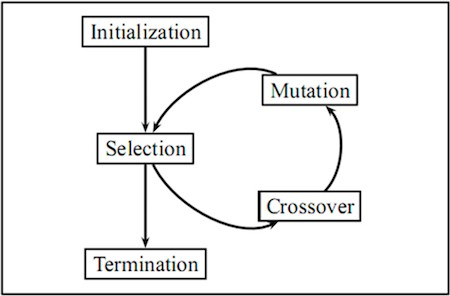
\includegraphics[scale=0.4]{Report/EAflow.png}\\
    Fig. 1: Flowchart of Evolutionary Algorithms
\end{center}

\subsection{NP-Completeness}
The NP-Completeness theory provides us with certain techniques to help prove that a given problem is difficult to solve, in a manner similar to other problems. By 'problems', we are referring to those which are widely accepted as unsolvable such as Traveling salesman problem or Knapsack problem. Decision problems, that are considered NP-Complete can not be solved in polynomial time, and we can, at best, find an approximate solution, with respect to our given resources.
\\
\\
NP-complete problems are "inherently intractable". To understand this term, let us first define strictly what we mean by 'problem' and 'solution'. A problem is a general question comprised of:
\begin{enumerate}
    \item A general description of the problem at hand.
    \item A statement on what properties the potential solution is required to answer. \cite{garey_johnson_2003}
\end{enumerate}
A solution is an answer or algorithm that can accurately and clearly solve the given problem. Looking back at the example of the Traveling Salesman Problem (TSP), the parameters of the problem are comprised of a set of cities, and the distances between different pairs of cities. The approximate solution aims to calculate a tour through all cities with the minimum possible distance possible. Emphasis is placed here on the word 'approximate', as with our strict definition of 'solution', we can say that there is no solution to the TSP. When there exists no solution to a problem, that problem is considered \textbf{inherently intractable}.

\subsubsection{NP-Completeness of the bandwidth minimization problem}
When it comes to computing matrices, especially larger, sparse ones, it is preferable to have all non-zero terms as close the the diagonal as possible. This is to enable easier manipulation of the matrices. The difference in absolute values of the most off-diagonal non-zero terms is referred to as the bandwidth of the matrix (see \hyperref[intro]{section 1.0})
\\
\\
Historically, there have been endeavours to decrease (see \cite{10.1145/800195.805928}, - \cite{sparse}), or minimize (see \cite{chen}, \cite{chen2}) the bandwidth of large, spares matrices, effectively, by permuating rows and columns. This has been translated to graph theory by Harary (see \cite{1973141}). 
Papadimitriou in his paper, proves that the minimization of the bandwidth of a matrix is an NP-complete problem. \cite{papadimitriou_1976}


\section{Conclusion}
The conclusion goes here.



% use section* for acknowledgment
\ifCLASSOPTIONcompsoc
  % The Computer Society usually uses the plural form
  \section*{Acknowledgments}
\else
  % regular IEEE prefers the singular form
  \section*{Acknowledgment}
\fi


The authors would like to thank Kopka, Helmut and Daly, Patrick W. \cite{10.5555/940746} for their publicly available \LaTeX document template.





\bibliographystyle{ieeetr}
\bibliography{refs.bib}




\end{document}
